% %
% main.tex
%

% notes = hide | show | only
\documentclass[xcolor=dvipsnames,dvip,notes=show,table]{beamer}

% Para crear una versión 'handout' (impresa)
%\documentclass[xcolor=pst,dvips,handout,notes=show]{beamer}

%
% cabeceras.tex
%

\usepackage[T1]{fontenc}

 \definecolor{ZurichBlue}{rgb}{.255,.41,.884}
 \beamertemplateshadingbackground{white!10}{white!10}
%\usepackage{beamerthemeWarsaw}

% \usepackage{longtable}
\usepackage{beamerthemeBoadilla}


%\usepackage{tikz,times}
\usetheme{boxes}
%\usepackage{handoutWithNotes}
\usepackage{pgfpages}
\pgfpagesuselayout{2 on 1}[a4paper,border shrink=5mm]


%\usecolortheme[named=OliveGreen]{structure} 
\setbeamertemplate{items}[ball] 
%\setbeamertemplate{blocks}[rounded][shadow=true] 
\setbeamertemplate{footline}[page number]
\addtocounter{framenumber}{-1}
%Handout



%\usepackage{beamertheme}
%\usepackage{beamerthemeshadow}
\useoutertheme[hooks]{tree}
 
% \setbeamertemplate{headline}[default] % The default is just an empty headline.
% \setbeamertemplate{headline}[infolines theme]
% \setbeamertemplate{headline}[miniframes theme]
% \setbeamertemplate{headline}[sidebar theme]
% \setbeamertemplate{headline}[smoothtree theme]
% \setbeamertemplate{headline}[smoothbars theme]
% \setbeamertemplate{headline}[tree]
\beamertemplatetransparentcovereddynamic
% spanish
\usepackage[spanish]{babel}
\usepackage[utf8]{inputenc}

% diagramas
%\usepackage{pst-eps,epstopdf}
\usepackage{pst-node}
%\usepackage{pst-all}
\usepackage{pst-blur}
%\usepackage{pst-tree}

% incrustaciones de código fuente
\usepackage{listings}

% matemáticas y símbolos
\usepackage{amsmath}
\usepackage{amssymb}
\usepackage[right]{eurosym}
\usepackage{ulem}

% colores
\usepackage{colortbl}

%\usepackage{algorithm2e}
%\usepackage{algorithm}
%\usepackage{algorithmic}

\lstset{language=[90]Fortran,
  basicstyle=\ttfamily,
  keywordstyle=\color{darkred},
  commentstyle=\color{green},
  frame=trBL,
  stringstyle=\color{violet},
  frameround=tttt,
  backgroundcolor=\color{lightyellow},
  morecomment=[l]{!\ }% Comment only with space after !
}


% 
% \lstset{%
%   language=Fortran,
% 	basicstyle=\footnotesize\sffamily,
% 	keywordstyle=\color{darkred}
%  	stringstyle=\color{violet}
%  	commentstyle=\color{blue}
%  	showspaces=false,
%  	showtabs=false,
%  	showstringspaces=false,
%  	frame=trBL,
%         frameround=tttt,
%         backgroundcolor=\color{lightyellow},
%  	extendedchars=true,
%  	numbers=none,
%         aboveskip=0.5cm,
%         belowskip=0.5cm,
%         xleftmargin=1cm,
%         xrightmargin=1cm,
% 	breaklines=true
% }
\definecolor{darkred}{rgb}{0.5, 0, 0}
\definecolor{violet}{rgb}{1, 0, 1}
\definecolor{lightyellow}{rgb}{1,1,0.8}


\usepackage{latexsym}
\usepackage{amsmath}
\usepackage{amssymb}
\usepackage{amsthm}

\usepackage{xspace}



\hyphenation{real}

\newrgbcolor{ColorEncabezadoTabla}{0.7 0.7 0.9}
\newrgbcolor{ColorFila1}{0.8 0.8 0.7}
\newrgbcolor{ColorFila2}{0.8 0.7 0.8}
\newrgbcolor{ColorTotal}{0.7 0.9 0.7}


% \usepackage{tikz,times}
% \usetikzlibrary{mindmap,backgrounds}



%%%%%%%%%%%%%%%%%%%%%%%%%%%%%%%%%%%%%%%%%%%%%%%%%%%%%%%%%%%%%%%%%%%%%%

\title[The RDFIndex approach | MTSR 2013]{Leveraging semantics to represent and compute quantitative indexes. \\ The RDFIndex approach.}
\author[Jose María Álvarez Rodríguez]{\textbf{Michalis Vafopoulos} (speaker) \\ and \\ Jose María Álvarez-Rodríguez}
\institute{MTSR 2013 | 7th Metadata and Semantics Research Conference \\ Main Track}


\date{}

\begin{document}

\frame{
\titlepage

}

\section{Introduction}

\frame{
  \frametitle{The Motivating example...} 
  
  
\begin{columns}[c] % the "c" option specifies center vertical alignment
\column{.5\textwidth} % column designated by a command


\begin{block}{Let's suppose that...}
 \begin{enumerate}
\item We want to create a ``Health index''...
\item ...to know which is the most ``healthy'' country.
\item ...to know which is the performance of the health expenditure .
\item ...to collect in just one value a set of indicators.
\item ...to make some new policy.
\end{enumerate}
\end{block}


\column{.5\textwidth}


\begin{figure}[htb]
\centering
	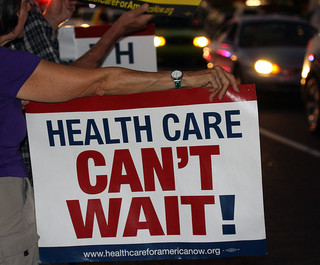
\includegraphics[width=4cm]{imgs/health}
%\caption{Modelo $5\star$ (W3C).}
\end{figure}

\end{columns}


}

\frame{
  \frametitle{The Motivating example...} 
  

\begin{block}{It is not a big deal because...}
 \begin{itemize}
\item We have the \textbf{``Health Index''} by an international network of physicians and researchers (\url{http://www.healthindex.com/}).
\item ...or the \textbf{``Health Index''} by the United Nations (\url{http://hdrstats.undp.org/en/indicators/72206.html}).
\item ...or the \textbf{``Ocean Health Index''} by an international collaborative effort (\url{http://www.oceanhealthindex.org/}).
\item ...or the indicators in the \textbf{World Bank} (\url{http://data.worldbank.org/topic/health}).
\item \ldots
\end{itemize}
\end{block}

}

\frame{
  \frametitle{The Motivating example...} 
 
   
\begin{exampleblock}{Benefits of using an index...}
 \begin{enumerate}
\item Creation of valuable data and information.
\item Generation of know-how to make some policy.
\item Re-use of a great effort and commitment by experts in some area.
\item Rank entities according to a quantitative value.
\item \ldots
\end{enumerate}
\end{exampleblock}

}

\frame{
  \frametitle{The Motivating example...} 
 
\scriptsize
\begin{alertblock}{Drawbacks of existing indexes...}<1->
 \begin{enumerate}
\item \textbf{Data heterogenity}: different datasources, formats and access protocols.
\item \textbf{Structure}: math models to aggregate some indicators that can change over time.
\item \textbf{Computation process}: observations are gathered and processed, \textit{somehow}, generating a final value.
\item \textbf{Documentation}: mutilingual and multicultural character of information.
\item \ldots
\end{enumerate}
\end{alertblock}

\begin{exampleblock}{..that imply the \textbf{necessity} of...}<2->
 \begin{enumerate}
\item \textbf{Accessing} \textbf{data} and information under a \textbf{common and shared data model}.
\item \textbf{Representing} the evolving \textbf{structure of the index}.
\item \textbf{Computing} the index to improve transparency.
\item Providing \textbf{context-aware documentation}: user-profile.
\item ... \textbf{Exploiting valuable data and metadata}.
\end{enumerate}
\end{exampleblock}

}


\frame{
  \frametitle{...but...Is it a common problem?} 
  

\begin{columns}[c] % the "c" option specifies center vertical alignment
\column{.5\textwidth} % column designated by a command


\begin{exampleblock}{...some indexes (per domain)...}
 \begin{enumerate}
\item Bibliography: the JCR and JSR, etc.
\item Government: the GDP, etc.
\item Web: the Webindex, etc.
\item Health: (the aforementioned ones).
\item Cloud: the CSC Cloud Usage Index, the VMWare index, the SMI index, etc.
\item ...to name a few per domain and creators.
\end{enumerate}
\end{exampleblock}


\column{.5\textwidth}


\begin{figure}[htb]
\centering
	
\includegraphics[width=5cm]{imgs/indexes}
%\caption{Modelo $5\star$ (W3C).}
\end{figure}

\end{columns}


}

\frame{
  \frametitle{Main Contributions} 
}


\section{Related Work}

\frame{
  \frametitle{Linked Open Data} 
}


\frame{
  \frametitle{Statistics and Linked Open Data} 
}


\section{The RDFIndex approach}

\frame{
  \frametitle{Overview} 
}

\frame{
  \frametitle{Example} 
}

\frame{
  \frametitle{Step 1: FIXME} 
}


\section{Use Case: the PublicSpending initiative}

\frame{
  \frametitle{Overview} 
}

\frame{
  \frametitle{The CORFU technique in Action...} 
}


\section{Evaluation}

\frame{
  \frametitle{Design of the experiment} 
}



\frame{
  \frametitle{Results} 
}


\section{Discussion}

\frame{
  \frametitle{Advantages} 
}


\frame{
  \frametitle{Restrictions} 
}



\section{Conclusions and Future Work}

\frame{
  \frametitle{Conclusions} 
}


\frame{
  \frametitle{Future Work} 
}


\section{Metadata and Information}

\frame{
  \frametitle{Acknowledgements} 
\begin{figure}[!htb]
\centering
 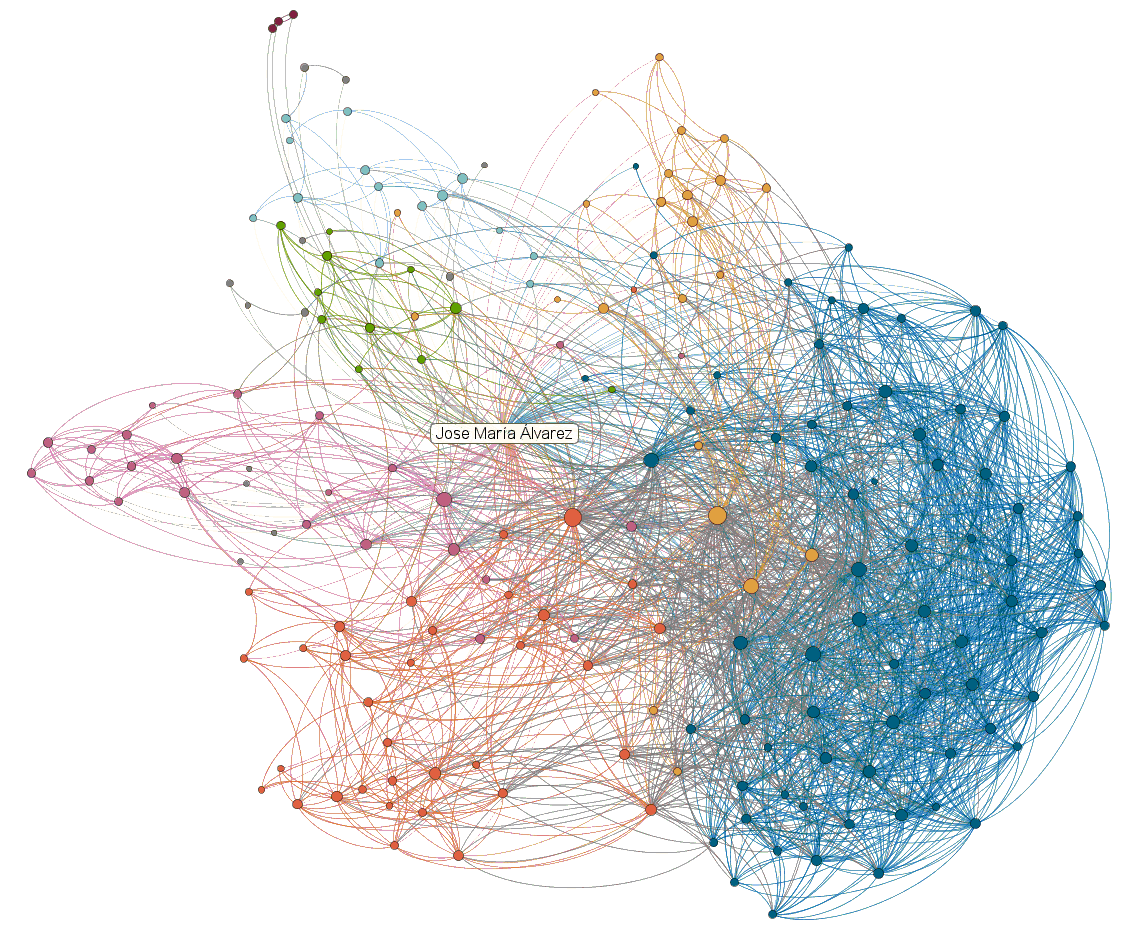
\includegraphics[width=9cm]{imgs/linkedin}
\end{figure}
}


\frame{
  \frametitle{Contact} 
}

\frame{
  \frametitle{Credits} 
}

\frame{
  \frametitle{References} 
}


\frame{
  \frametitle{Thank you...} 
}


\frame{
\titlepage

}


% %%%%%%%%%%%%%%%%%%%%%%%%%%%%%%%%%%%%%%%%%%%%%%%%%%%%%%%%%%%%%%%%%%%%%%

\end{document}
